%%%%%%%%%%%%%%%%%%%%%%%%%%%%%%%
%%%%%%%%%%%%%%%%%%%%%%%%%%%%%%%
\chapter{Methods\label{ch:methods}}
%%%%%%%%%%%%%%%%%%%%%%%%%%%%%%%
%Section comments: There were more changes related to objective language and directional words. There is a missing term near line 13.
The system identification of rigid body ship dynamics can be simplified into parameter estimation if parameterized physical models can be assumed. Parameter estimations for roll motion and manoeuvring are presented in \ref{sec:_roll} and \ref{sec:_VMM}. System identification can be performed by selecting the most appropriate model from a collection of candidate models.

\section{Roll model parameter estimation} \label{sec:_roll}
\noindent Parameter estimation can be applied to identify the roll damping parameters ($B_1$, $B_2$, $B_3$) and stiffness parameters ($C_1$, $C_3$, $C_5$) in the parameterized roll motion models from the previous chapter (\autoref{eq:roll_decay_equation_himeno_linear}, \autoref{eq:roll_decay_equation_himeno_quadratic_b} and \autoref{eq:roll_decay_equation_cubic}). These equations do not have unique solutions because each equation can be multiplied by an arbitrary factor to obtain a new valid solution. Inertia is therefore excluded to obtain unique solutions. This is achieved by normalizing the equations by the total roll inertia $A_{44}$, as seen in \autoref{eq:roll_decay_nonedim_a44}, for the linear model.

\begin{equation} \label{eq:roll_decay_nonedim_a44}
\ddot{\phi} + \frac{B_{1}}{A_{44}} \dot{\phi} + \frac{C_{1}}{A_{44}} \phi = 
\ddot{\phi} + B_{1A} \dot{\phi} + C_{1A} \phi = 0
\end{equation}

\noindent The identified normalized damping and stiffness parameters $B_{1A}$ and $C_{1A}$ can be expressed in dimensional units by multiplication with the normalization factor $A_{44}$. If $A_{44}$ is unknown before hand, it can be calculated using \autoref{eq:A_44_eq} \cite{piehl_ship_2016}, assuming that the meta center height $GM$ is known.
\begin{equation} \label{eq:A_44_eq}
A_{44} = \frac{GM g m}{\omega_{0}^{2}}
\end{equation}


\noindent The frequency $\omega_0$ can be obtained with Fast Fourier transform (FFT) of the roll signal. 
Two methods have been investigated: the ``derivation approach'', referred to in \parencite{imo_1200_2006}, and the ``integration approach'' used in \cite{soder_assessment_2019}. 

\subsection{Derivation approach}\label{sec:derivation_approach}
In the derivation approach, \autoref{eq:roll_decay_nonedim_a44} is treated as a linear regression problem, where the states ($\phi$, $\dot{\phi}$, $\ddot{\phi}$) are known and the parameters $B_1$ and $C_1$ must be regressed. Only roll angle $\phi$ is known from the experimental data, which means that the velocity and acceleration $\dot{\phi}$, $\ddot{\phi}$ also must be estimated (note that this is done with numerical differentiation in Paper \ref{pap:rolldamping} and with the extended Kalman filter (EKF) in Paper \ref{pap:pit}).
A least squares fit must be applied to the roll motion equation to identify the damping and stiffness parameters.

\subsection{Integration approach}\label{sec:integration_approach}
In the integration approach, \autoref{eq:roll_decay_nonedim_a44} is solved as an ordinary differential equation (ODE) for many estimated sets of parameters until the solution converges. This method is time-consuming, and convergence is not guaranteed. However, the advantage is that only roll angle $\phi$ is needed.

\section{Manoeuvring model parameter estimation} \label{sec:_VMM}
In the proposed parameter estimation, a manoeuvring model is used to solve the reversed manoeuvring problem. The problem may consist of predicting unknown forces from known manoeuvring model test data. The hydrodynamic derivatives in the manoeuvring model can be identified through regression of the force polynomials on forces predicted with inverse dynamics (see \autoref{\detokenize{03.01_inverse_dynamics::doc}}).
The measurement noise must be removed prior to the regression of hydrodynamic derivatives in the manoeuvring model. This is conducted by an extended Kalman filter (EKF) and a Rauch Tung Striebel (RTS) smoother (see \autoref{sec:datacleaning}). The EKF requires an accurate manoeuvring model as the predictor.
Therefore, the accurate manoeuvring model is both the input and output of the method. A linear manoeuvring model that includes hydrodynamic derivatives estimated with semi-empirical formulas (\autoref{app:initial_estimates}) is used as the initial predictor. Once the regressed manoeuvring model has been obtained, the parameter estimation can be refined, using the regressed manoeuvring model as the predictor model in the EKF, to improve the filter and obtain a more accurate manoeuvring model. The method is summarized in Fig.\ref{fig:greyvmm} and can be repeated several times (indicated by the dashed arrow) for improved accuracy. 

\begin{figure}[H]
    
    \centering
    \begin{tikzpicture}[node distance=1.5cm]
    %\draw (0,0) rectangle (10,10); %create a bounding box to reserve space
    \node (data) [io] {\footnotesize Model test data: $x$, $\delta$, thrust};
    
    \node (EKF) [process, right of=data, xshift=3.0cm] {\footnotesize EFK + RTS};
    \node (predictor) [process, right of=EKF, xshift=2.0cm]{\footnotesize Predictor};
    \node (VMM) [io, right of=predictor, xshift=1.0cm] {\footnotesize initial model};
    
    \node (data_clean) [io, below of=EKF] {\footnotesize \(x,\dot{x},\ddot{x}, \delta, thrust\)};
    
    \node (black-box) [black-box, below of=data_clean] {\footnotesize Regression};
    
    \node (X_D) [io, left of=black-box, xshift=-0.70cm, yshift=0.7cm]{\footnotesize \(X_D\)};
    \node (Y_D) [io, left of=black-box, xshift=-0.70cm, yshift=0cm]{\footnotesize \(Y_D\)};
    \node (N_D) [io, left of=black-box, xshift=-0.70cm, yshift=-0.7cm]{\footnotesize \(N_D\)};
    
    \node (white-box) [white-box, left of=Y_D, xshift=-1.00cm] {\footnotesize Inverse dynamics};
    
    
    %
    %
    \node (coefficients) [io, right of=black-box, xshift=2.0cm] {\footnotesize model$\left(Y_{uv},N_{\delta},...\right)$};
    
    \draw [arrow] (data) -- (EKF);
    \draw [arrow] (predictor) -- (EKF);
    \draw [arrow] (VMM) -- (predictor);
    \draw [arrow] (EKF) -- (data_clean);
    
    \draw [arrow] (data_clean) -| (white-box);
    \draw [arrow] (data_clean) -- (black-box);
    
    \draw [arrow] (white-box) -- (X_D);
    \draw [arrow] (white-box) -- (Y_D);
    \draw [arrow] (white-box) -- (N_D);
    
    \draw [arrow, shorten >=0.5cm] (X_D) -- (black-box);
    \draw [arrow, shorten >=0.2cm] (Y_D)  -- (black-box);
    \draw [arrow, shorten >=0.5cm] (N_D)  -- (black-box);
    
    \draw [arrow] (black-box)  -- (coefficients);
    \draw [arrow, dashed] (coefficients)  -- (predictor);
    
    \end{tikzpicture}
    \caption{Method to estimate the manoeuvring model hydrodynamic derivatives}
    \label{fig:greyvmm}
\end{figure}

\noindent Using semi-empirical formulas (\autoref{app:initial_estimates}) for the initially estimated manoeuvring model adds prior knowledge about the ship dynamics to the regression. An example, with simulation results from the steps in the iteration, is presented in \hyperref[\detokenize{01.01_method:iterations}]{Fig.\@\ref{\detokenize{01.01_method:iterations}}}.


\begin{figure}[H]
    \centering
    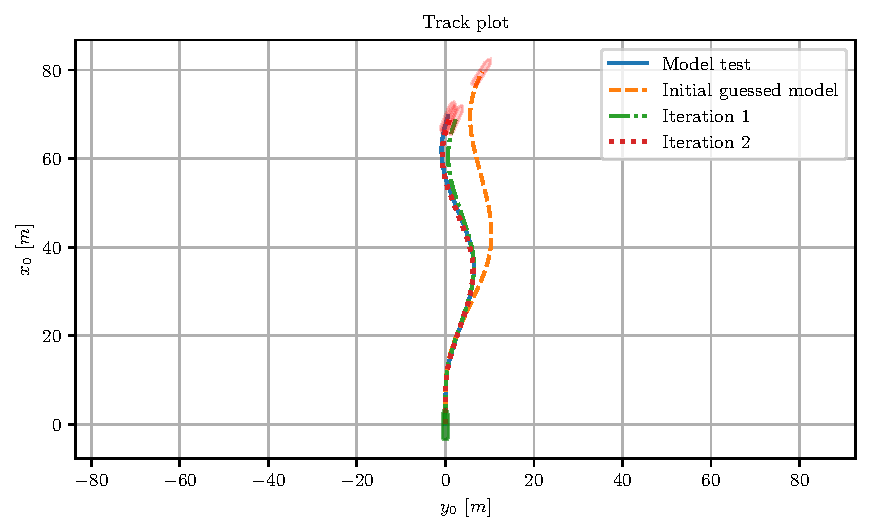
\includegraphics[width=\textwidth]{kappa/images/0.pdf}
    \caption{Simulation with: initial model and first and second iteration of the parameter estimation method.}
    \label{\detokenize{01.01_method:iterations}}
\end{figure}

\subsection{Inverse dynamics and regression}
\label{\detokenize{03.01_inverse_dynamics:inverse-dynamics-and-regression}}\label{\detokenize{03.01_inverse_dynamics::doc}}

Each manoeuvring model has some hydrodynamic functions \(X_D(u,v,r,\delta,thrust)\), \(Y_D(u,v,r,\delta,thrust)\), \(N_D(u,v,r,\delta,thrust)\) that are defined as polynomials. The hydrodynamic derivatives in these polynomials can be identified with force regression of measured forces and moments. The measured forces and moments are usually taken from captive model tests (CMT), planar motion mechanism (PMM) tests, or virtual captive tests (VCT). However, motions are recorded when the ship is free in all degrees of freedom. Hence, forces and moments causing ship motion must be estimated by solving the inverse dynamics problem.
The inverse dynamics problem is solved by restructuring the system equation (\autoref{equation:02.01_manoeuvring models:eqacc}) to get the hydrodynamics functions on the left-hand side. If the mass and inertia of the ship with added masses: \(X_{\dot{u}}\), \(Y_{\dot{v}}\), \(Y_{\dot{r}}\), \(N_{\dot{v}}\), and \(N_{\dot{r}}\) are known; the forces in the Prime system can be calculated using \autoref{equation:03.01_inverse_dynamics:eqxd}, \autoref{equation:03.01_inverse_dynamics:eqyd}, and \autoref{equation:03.01_inverse_dynamics:eqnd}.
These forces can be used to regress the hydrodynamic derivatives through the ordinary least square (OLS) method. If the added masses are unknown, they can be calculated using potential flow methods or semi-empirical methods (\autoref{app:initial_estimates}). 
\begin{equation}\label{equation:03.01_inverse_dynamics:eqxd}
\begin{split}\displaystyle \operatorname{X_{D}'}{\left(u',v',r',\delta,thrust' \right)} = - X_{\dot{u}}' \dot{u}' + \dot{u}' m' - m' r'^{2} x_{G}' - m' r' v'\end{split}
\end{equation}\begin{equation}\label{equation:03.01_inverse_dynamics:eqyd}
\begin{split}\displaystyle \operatorname{Y_{D}'}{\left(u',v',r',\delta,thrust' \right)} = - Y_{\dot{r}}' \dot{r}' - Y_{\dot{v}}' \dot{v}' + \dot{r}' m' x_{G}' + \dot{v}' m' + m' r' u'\end{split}
\end{equation}\begin{equation}\label{equation:03.01_inverse_dynamics:eqnd}
\begin{split}\displaystyle \operatorname{N_{D}'}{\left(u',v',r',\delta,thrust' \right)} = I_{z}' \dot{r}' - N_{\dot{r}}' \dot{r}' - N_{\dot{v}}' \dot{v}' + \dot{v}' m' x_{G}' + m' r' u' x_{G}'\end{split}
\end{equation}

\noindent An example that includes forces calculated with inverse dynamics from motions in a turning circle test can be seen in \hyperref[\detokenize{03.01_inverse_dynamics:fig-inverse}]{Fig.\@ \ref{\detokenize{03.01_inverse_dynamics:fig-inverse}}}. The forces have been converted to SI units.

\begin{figure}[H]
    \centering
    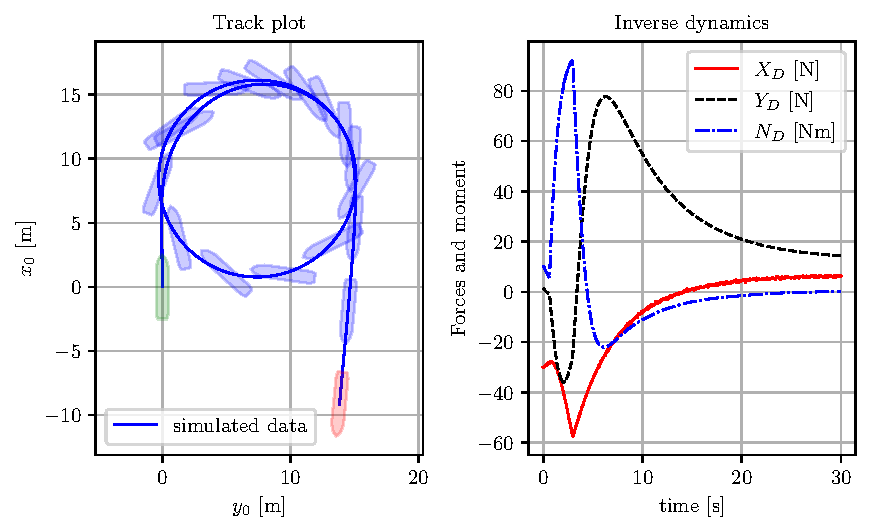
\includegraphics[width=\textwidth]{kappa/images/1.pdf}
    \caption{Forces and moments calculated with inverse dynamics on data from a turning circle test.}
    \label{\detokenize{03.01_inverse_dynamics:fig-inverse}}
\end{figure}

\subsection{Data cleaning}
\label{sec:datacleaning}
It is possible to do an exact parameter estimation on flawless (simulated) data with no noise (see Paper \ref{pap:pit}). However, such data from physical experiments does not exist in reality. The measured data will always contain process noise and measurement noise. In order to mitigate the effects of noise, the data is pre-processed using the extended Kalman filter (EKF) \cite{brown_introduction_1997} and the Rauch Tung Striebel (RTS) smoother \cite{rauch_maximum_1965}, which are both presented below.
EKF is an extension of the Kalman filter (KF) that is used to work on nonlinear systems such as the manoeuvring models. The premise is that noise can be neglected if it has no rational physical explanation. For instance, if noisy measurement data would be  completely correct, that would mean that large ship vibrations must have originated from large high frequency forces considering the large mass of the ship. A prior understanding of the dynamics suggests that these forces are not present. Therefore, the noise should be considered as measurement noise and should be removed. Low-pass filtering is commonly used to remove noise; motions above a cutoff frequency are considered unphysical measurement noise. The problem with low-pass filtering is that choosing the cutoff frequency is difficult. It is often  either too low (removing some of the signal) or too high (keeping some unfiltered measurement noise in the data). The Kalman filter has a predictor model, a manoeuvring model in this case, that continuously estimates the system’s state that runs parallel with the measurement data. The filter estimates the current state as a combination of the measurement data and the predictor model estimate based on the possible validity of the data and the model. If the data has low noise, the estimate is closer to that data. Conversely, if the model provides very accurate predictions, then that estimate is closer to the model.
The system’s inverse dynamics require everything about the state (positions, velocities, and accelerations) to be known. Only positions are known from the measurements, but the velocities and accelerations are instead estimated by the EKF.
The EKF is recursive and can be ran online; it continuously makes new estimates as new measurements arrive. The EKF uses passed measurements to estimate states in the near future. This property is commonly used for online applications such as autopilots or autonomous ships. This restriction is unnecessary for the estimation for already existing data, where an entire time series of existing measurements is available. The knowledge of both past and future data can be used to improve the filter. An EKF filter can include future time steps by adding the RTS smoother after the filter. The RTS smoother is an algorithm that runs the EKF backward to account for future time steps.

\subsection{Regression}
Finding the hydrodynamic derivatives can be defined as a linear regression problem:
\begin{equation}\label{equation:03.01_inverse_dynamics:eqregression}
\begin{split}y = X\gamma + \epsilon\end{split}
\end{equation}

\noindent A model for the hydrodynamic forces must first be assumed.
The label vector \(y\) and feature matrix \(X\) in the regression problem in \autoref{equation:03.01_inverse_dynamics:eqregression} can now be calculated based on the assumed model. For example: the label in the regression of the surge degree of freedom for the MAVMM can be calculated using the inverse dynamics force, which is expressed with primed units:
\begin{equation}\label{equation:03.01_inverse_dynamics:diff_eq_X_y}
\begin{split}\displaystyle y = - X_{\dot{u}} \dot{u}' + \dot{u}' m' - m' r'^{2} x_{G'} - m' r' v'\end{split}
\end{equation}

\noindent The feature matrix \(X\) is expressed as:
\begin{equation}\label{equation:03.01_inverse_dynamics:diff_eq_X_X}
\begin{split}\displaystyle X = \left[\begin{matrix}thrust' & u' & \delta^{2} & r'^{2} & u'^{2} & r' v'\end{matrix}\right]\end{split}
\end{equation}

\noindent The regressed hydrodynamic derivatives are stored in the \(\gamma\) vector:
\begin{equation}\label{equation:03.01_inverse_dynamics:diff_eq_X_beta}
\begin{split}\displaystyle \gamma = \left[\begin{matrix}X_{T}\\X_{u}\\X_{\delta\delta}\\X_{rr}\\X_{uu}\\X_{vr}\end{matrix}\right]\end{split}
\end{equation}

\noindent The hydrodynamic derivatives in the manoeuvring model are treated as Gaussian random variables when conducting the ordinary least squares (OLS) regression. The hydrodynamic derivatives in the manoeuvring model are usually taken as the mean value of each regressed random variable, which is the most likely estimate. The regression result can be expressed with a multivariate Gaussian distribution, which is defined by the regression’s mean values and covariance matrix. The multivariate Gaussian distribution can be used to conduct Monte Carlo simulations in the study of alternative realizations of the regression.


Strong multicollinearity is a documented problem for the manoeuvring models \cite{luo_parameter_2016, wang_quantifying_2018}.
The thrust coefficient \(X_T\) in the hydrodynamic function \(X_D\) in \autoref{equation:02.01_manoeuvring models:eqxabkowitz} introduces multicollinearity to the regression. This coefficient can instead be calculated from the thrust deduction factor \(t_{df}\):
\begin{equation}\label{equation:03.01_inverse_dynamics:eqXthrust}
\begin{split}\displaystyle X_{T} = 1 - t_{df}\end{split}
\end{equation}

\noindent The \(X_T\) coefficient is excluded from the regression by moving it to the left-hand side of the regression equation \autoref{equation:03.01_inverse_dynamics:eqregression}:
\begin{equation}\label{equation:03.01_inverse_dynamics:eqexclude}
\begin{split}y-X_T \cdot thrust = X \gamma + \epsilon\end{split}
\end{equation}

\noindent Rudder coefficients (\(Y_R\)) from \(Y_D\) equation \autoref{equation:02.01_manoeuvring models:eqyabkowitz}, such as \(Y_{\delta}\) and \(Y_{\delta T}\), have also been excluded by assuming a connection with their \(N_D\) equation counterpart through the rudder lever arm \(x_r\):
\begin{equation}\label{equation:03.01_inverse_dynamics:eqyr}
\begin{split}\displaystyle Y_{R} = \frac{N_{R}}{x_{r'}}\end{split}
\end{equation}

\subsection{Model development process}
\label{sec:model_development_process}
The aim of developing a manoeuvring model with parameter estimation is to develop a model that can generalize outside the known data. The method presented in this thesis is assessed with the hold-out evaluation \cite{sammut_holdout_2017}. The data in this evaluation is divided into three sets: the training set, the validation set, and the test set. The development process can be seen in \autoref{fig:model_development_process}.

\begin{figure}[H]
\centering
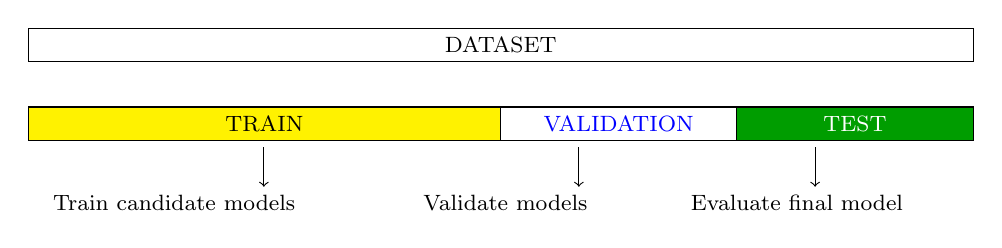
\begin{tikzpicture}

\node (dataset)[rectangle,
    anchor=west,
    draw,
    text = black,
    minimum width=12cm,
    fill = white] at (0, 0) {\footnotesize DATASET};

\node (train)[rectangle,
    draw,
    anchor=west,
    text = black,
    minimum width=6cm,
    fill = yellow] at (0, -1cm) {\footnotesize TRAIN};

\node (validation)[rectangle,
    draw,
    anchor=west,
    text = blue,
    minimum width=3cm,
    fill = white] at (6cm, -1cm) {\footnotesize VALIDATION};

\node (test)[rectangle,
    draw,
    anchor=west,
    text = white,
    minimum width=3cm,
    fill = black!15!green!255] at (9cm, -1cm){\footnotesize TEST};
    
\node (train_multiple)[rectangle,
    draw,
    anchor=west,
    text = black,
    draw = none,
    fill = none] at (0.2cm, -2cm){\footnotesize Train candidate models};
    
\node (validate_models)[rectangle,
    draw,
    anchor=west,
    text = black,
    draw = none,
    fill = none] at (4.9cm, -2cm){\footnotesize Validate models};
    
\node (evaluate_models)[rectangle,
    draw,
    anchor=west,
    text = black,
    draw = none,
    fill = none] at (8.3cm, -2cm) {\footnotesize Evaluate final model};

\draw[->] (3,-1.3) -- (3,-1.8);
\draw[->] (7,-1.3) -- (7,-1.8);
\draw[->] (10,-1.3) -- (10,-1.8);



\end{tikzpicture}
\caption{Model development process with hold-out evaluation}
\label{fig:model_development_process}
\end{figure}

\noindent The purpose of the training set is to train all the candidate models using the proposed parameter estimation method. The validation set is then used to select the most effective candidate model. The training and validation sets are then joined to train the selected model as the final model. The final model is used for predicting the test set, which is used to evaluate the accuracy of the model. These three sets are not divided randomly;  they are divided to assess the model’s extrapolation ability. The data sets are therefore split to have the smallest yaw rates, drift-angles, and rudder-angles in the training set; the medium values in the validation set; and the largest values in the test set, which can be seen in \autoref{fig:wpcc_datasets} in the next chapter.


